\documentclass[11pt]{article}

\usepackage[utf8]{inputenc}
\usepackage[T1]{fontenc}
\usepackage{lmodern}
\usepackage[margin=1in]{geometry}
\usepackage{setspace}
\usepackage{booktabs}
\usepackage{longtable}
\usepackage{tabularx}
\usepackage{multirow}
\usepackage{array}
\usepackage{graphicx}
\usepackage{float}
\usepackage{caption}
\usepackage{makecell}
\usepackage{subcaption}
\usepackage{amsmath}
\usepackage{siunitx}
\usepackage{hyperref}
\usepackage{xcolor}
\usepackage{tikz}
\usepackage{pgfplots}
\pgfplotsset{compat=1.18}
\usetikzlibrary{arrows.meta,positioning,shapes.geometric,fit,calc}

\graphicspath{{./fig/dashboard/}{./fig/eda/}}

\title{Traceable Predictive Maintenance for NASA C-MAPSS:\\
An End-to-End PHM System with Calibrated RUL Prediction, Deterministic Risk Logic, and Interactive Scenario Analysis}
\author{CMAPSS-PHM Project}
\date{April 2026}

\begin{document}
\maketitle
\onehalfspacing

\begin{abstract}
This paper presents an end-to-end predictive maintenance application built on the NASA C-MAPSS benchmark. The system combines a multi-model predictive layer for Remaining Useful Life (RUL) estimation, a deterministic agent layer for risk scoring and maintenance recommendations, and a dashboard layer for decision presentation, scenario analysis, and technical auditability. Candidate models include Random Forest, HistGradientBoosting, LSTM, and GRU. Although GRU achieved the best raw RMSE, the deployed champion is Random Forest because it offered stronger stability and integration readiness. The application augments point predictions with calibrated confidence bands, converts them into traceable risk and recommendation outputs, and exposes the full workflow through interactive user and technical-audit views. The result is both a scientific study on C-MAPSS PHM and an implemented AI system suitable for reproducible deployment-oriented evaluation.
\end{abstract}

\section{Introduction}
Remaining Useful Life (RUL) estimation is a core task in prognostics and health management (PHM), but benchmark-oriented studies often stop at predictive model scores. Real maintenance systems need uncertainty handling, deterministic decision logic, scenario analysis, explainability, and traceability in addition to point estimates. This work addresses that integration gap by implementing and evaluating a layered PHM stack over NASA C-MAPSS data \cite{nasa_cmapss_guide,saxena2008damage}.

\textbf{Contributions.}
\begin{itemize}
  \item A calibrated and benchmarked predictive layer with champion selection driven by accuracy and operational constraints.
  \item A deterministic agent layer that maps predictive outputs to auditable risk and recommendation decisions.
  \item A dashboard layer that operationalizes summary, analysis, scenarios, and technical-audit workflows.
  \item A reproducible artifact package linking data, code, models, contracts, and runtime traces.
\end{itemize}

\section{Related Work}
Research around C-MAPSS has heavily emphasized predictive performance, especially with sequence models such as LSTM and GRU \cite{ramasso2014prognostics,zheng2017lstm}. Tree-based methods remain strong tabular baselines for robustness and low-latency deployment. PHM deployment literature additionally highlights the importance of uncertainty communication, actionability, and governance in safety-critical settings \cite{sikorska2011prognostic,lee2014service}. This paper positions itself between benchmark modeling and deployable PHM decision-support systems.

\section{Dataset and Engine Context}
\subsection{NASA C-MAPSS problem setting}
C-MAPSS represents multivariate run-to-failure trajectories generated from a turbofan simulation framework \cite{nasa_cmapss_guide}. Each row contains a unit identifier, cycle index, three operational settings, and sensor measurements. The four benchmark subsets differ in operating-condition and fault-mode complexity, summarized in Table~\ref{tab:cmapss_subsets}.

\begin{table}[H]
\centering
\caption{CMAPSS subsets and problem structure.}
\label{tab:cmapss_subsets}
\begin{tabular}{lcccc}
\toprule
Subset & Train units & Test units & Conditions & Fault modes \\
\midrule
FD001 & 100 & 100 & 1 (sea level) & 1 (HPC) \\
FD002 & 260 & 259 & 6 & 1 (HPC) \\
FD003 & 100 & 100 & 1 (sea level) & 2 (HPC + Fan) \\
FD004 & 248 & 249 & 6 & 2 (HPC + Fan) \\
\bottomrule
\end{tabular}
\end{table}

\subsection{Engine schematic context}
Figure~\ref{fig:engine_schematic} provides a conceptual turbofan degradation and monitoring view aligned with the NASA C-MAPSS guide. Operational settings and sensor channels define the context in which degradation patterns are observed cycle by cycle.

% \begin{figure}[H]
% \centering
% \resizebox{\textwidth}{!}{%
% \begin{tikzpicture}[
%   x=1cm,
%   y=1cm,
%   module/.style={draw, rounded corners=2pt, minimum height=0.9cm, minimum width=1.45cm, align=center, fill=blue!6},
%   side/.style={draw, rounded corners=2pt, minimum height=0.9cm, minimum width=1.6cm, align=center, fill=gray!8},
%   signal/.style={draw, rounded corners=3pt, minimum height=0.95cm, text width=3.7cm, align=center, fill=green!10},
%   arrow/.style={-Latex, thick},
%   sense/.style={-Latex, semithick},
%   every node/.style={font=\small}
% ]
% % Gas-path layout synthesised from the original C-MAPSS engine and module diagrams
% \node[side]   (ambient)      at (0.0,0.0)   {Ambient};
% \node[module] (inlet)        at (1.8,0.0)   {Inlet};
% \node[module] (fan)          at (3.4,0.0)   {Fan};
% \node[side]   (splitter)     at (5.2,0.0)   {Splitter};
% \node[side]   (bypasspath)   at (7.7,1.25)  {Bypass\Path};
% \node[side]   (bypassnozzle) at (10.5,1.25) {Bypass\Nozzle};
% \node[module] (lpc)          at (7.0,-1.15) {LPC};
% \node[module] (hpc)          at (8.8,-1.15) {HPC};
% \node[module] (burner)       at (11.1,-1.15){Burner};
% \node[module] (hpt)          at (13.2,-1.15){HPT};
% \node[module] (lpt)          at (15.0,-1.15){LPT};
% \node[side]   (corenozzle)   at (17.5,-1.15){Core\Nozzle};
% \node[module, minimum width=1.0cm] (fuel) at (9.9,-2.45) {Fuel};

% % Flow arrows
% \draw[arrow] (ambient) -- (inlet);
% \draw[arrow] (inlet) -- (fan);
% \draw[arrow] (fan) -- (splitter);
% \draw[arrow] (splitter.east) -- ++(0.35,0) |- (bypasspath.west);
% \draw[arrow] (bypasspath.east) -- (bypassnozzle.west);
% \draw[arrow] (splitter.east) -- ++(0.35,0) |- (lpc.west);
% \draw[arrow] (lpc) -- (hpc);
% \draw[arrow] (hpc) -- (burner);
% \draw[arrow] (fuel.north) -- ++(0,0.25) -| (burner.south);
% \draw[arrow] (burner) -- (hpt);
% \draw[arrow] (hpt) -- (lpt);
% \draw[arrow] (lpt) -- (corenozzle);

% % Simulation envelope
% \node[draw, dashed, rounded corners, fit=(ambient)(inlet)(fan)(splitter)(bypasspath)(bypassnozzle)(lpc)(hpc)(burner)(hpt)(lpt)(corenozzle)(fuel), inner sep=9pt, label={[yshift=0.45cm]above:{\normalsize Engine simulation core}}] (env) {};

% % Monitoring context blocks below the simulator
% \node[signal] (ops)  at (4.9,-4.0)  {Operational settings\[-1mm]\scriptsize altitude, Mach, throttle / operating regime};
% \node[signal] (sens) at (9.9,-4.0)  {Sensor stream\[-1mm]\scriptsize 21 measured channels from the simulated engine};
% \node[signal] (traj) at (14.9,-4.0) {Trajectory context\[-1mm]\scriptsize dataset, unit, cycle};

% % Monitoring arrows
% \draw[sense] (ops.north)  -- ++(0,0.35) -| (fan.south);
% \draw[sense] (ops.north)  -- ++(0,0.35) -| (splitter.south);
% \draw[sense] (sens.north) -- ++(0,0.35) -| (hpc.south);
% \draw[sense] (sens.north) -- ++(0,0.35) -| (burner.south);
% \draw[sense] (sens.north) -- ++(0,0.35) -| (hpt.south);
% \draw[sense] (traj.north) -- ++(0,0.35) -| (lpt.south);
% \draw[sense] (traj.north) -- ++(0,0.35) -| (corenozzle.south);
% \end{tikzpicture}%
% }
% \caption{Conceptual C-MAPSS monitoring schematic used in this study. The upper gas-path layout follows the closed-loop turbofan module connectivity described for the C-MAPSS simulator (ambient, inlet, fan, splitter, bypass path/nozzle, LPC, HPC, burner, HPT, LPT, core nozzle), while the lower blocks show the monitoring context consumed by the PHM pipeline: operational settings, sensor channels, and trajectory identifiers. Synthesized from the C-MAPSS engine and layout diagrams in Saxena et al. and the NASA C-MAPSS documentation.}
% \label{fig:engine_schematic}
% \end{figure}

\begin{figure}[H]
\centering
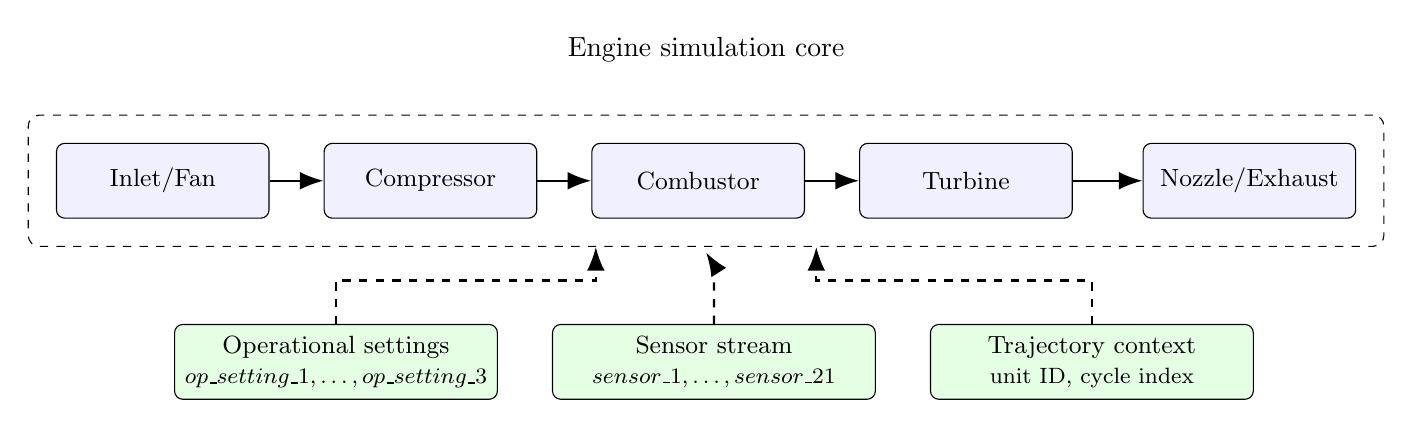
\begin{tikzpicture}[
  font=\small,
  >=Latex,
  block/.style={
    draw,
    rounded corners=3pt,
    minimum width=2.7cm,
    minimum height=0.95cm,
    align=center,
    fill=blue!6
  },
  signal/.style={
    draw,
    rounded corners=3pt,
    minimum width=4.1cm,
    minimum height=0.95cm,
    align=center,
    fill=green!10
  },
  flow/.style={
    -{Latex[length=3mm]},
    thick
  },
  info/.style={
    -{Latex[length=3mm]},
    thick,
    dashed
  }
]

%-----------------------------
% Engine core blocks
%-----------------------------
\node[block] (inlet) at (0,0) {Inlet/Fan};
\node[block] (comp)  at (3.4,0) {Compressor};
\node[block] (comb)  at (6.8,0) {Combustor};
\node[block] (turb)  at (10.2,0) {Turbine};
\node[block] (nozz)  at (13.8,0) {Nozzle/Exhaust};

\draw[flow] (inlet) -- (comp);
\draw[flow] (comp) -- (comb);
\draw[flow] (comb) -- (turb);
\draw[flow] (turb) -- (nozz);

%-----------------------------
% Dashed container
%-----------------------------
\node[
  draw,
  dashed,
  rounded corners=4pt,
  fit=(inlet)(comp)(comb)(turb)(nozz),
  inner sep=10pt,
  label={[yshift=0.55cm]above:\normalsize Engine simulation core}
] (enginebox) {};

%-----------------------------
% Input/context layer
%-----------------------------
\node[signal] (ops)   at (2.2,-2.3) {Operational settings\\{\footnotesize $op\_setting\_1,\dots,op\_setting\_3$}};
\node[signal] (sens)  at (7.0,-2.3) {Sensor stream\\{\footnotesize $sensor\_1,\dots,sensor\_21$}};
\node[signal] (cycle) at (11.8,-2.3) {Trajectory context\\{\footnotesize unit ID, cycle index}};

%-----------------------------
% Information links to the engine core
%-----------------------------
\draw[info] (ops.north)   -- ++(0,0.55) -| ([xshift=-1.4cm]enginebox.south);
\draw[info] (sens.north)  -- ++(0,0.75) -- ([yshift=-2pt]enginebox.south);
\draw[info] (cycle.north) -- ++(0,0.55) -| ([xshift=1.4cm]enginebox.south);

\end{tikzpicture}
\caption{Conceptual C-MAPSS turbofan monitoring schematic, adapted from the NASA C-MAPSS user-guide context.}
\label{fig:engine_schematic}
\end{figure}

\section{Methodology}
\subsection{Preprocessing and feature policy}
Preprocessing removes low-variance variables, fits a training-only standard scaler, and preserves both raw and capped RUL policies. Table~\ref{tab:features} summarizes the selected and removed feature sets used by the deployed predictive pipeline.

\begin{table}[H]
\centering
\caption{Selected vs removed low-variance features.}
\label{tab:features}
\begin{tabularx}{\textwidth}{>{\raggedright\arraybackslash}X>{\raggedright\arraybackslash}X}
\toprule
Selected predictive features (16) & Removed low-variance features (8) \\
\midrule
\texttt{op\_setting\_1}, \texttt{op\_setting\_2}, \texttt{sensor\_2}, \texttt{sensor\_3}, \texttt{sensor\_4}, \texttt{sensor\_7}, \texttt{sensor\_8}, \texttt{sensor\_9}, \texttt{sensor\_11}, \texttt{sensor\_12}, \texttt{sensor\_13}, \texttt{sensor\_14}, \texttt{sensor\_15}, \texttt{sensor\_17}, \texttt{sensor\_20}, \texttt{sensor\_21} &
\texttt{op\_setting\_3}, \texttt{sensor\_1}, \texttt{sensor\_5}, \texttt{sensor\_6}, \texttt{sensor\_10}, \texttt{sensor\_16}, \texttt{sensor\_18}, \texttt{sensor\_19} \\
\bottomrule
\end{tabularx}
\end{table}

\subsection{Candidate model portfolio}
Table~\ref{tab:model_matrix} summarizes the candidate-model roles.

% \begin{table}[H]
% \centering
% \caption{Candidate models and intended roles (T3).}
% \label{tab:model_matrix}
% \begin{tabularx}{\textwidth}{l l X l}
% \toprule
% Model family & Input shape & Core strengths & Role \\
% \midrule
% RandomForestRegressor & Row tabular & Robust baseline, fast iteration, stable serving & Baseline/champion candidate \\
% HistGradientBoostingRegressor & Row tabular & Competitive baseline, efficient training & Baseline/fallback candidate \\
% LSTM & Windowed sequence & Temporal degradation modeling & Sequence challenger \\
% GRU & Windowed sequence & Strong temporal pattern capture & Sequence challenger \\
% \bottomrule
% \end{tabularx}
% \end{table}

\begin{table}[H]
\centering
\caption{Candidate models and intended roles.}
\label{tab:model_matrix}
\begin{tabular}{p{3.6cm} p{3.0cm} p{5.2cm} p{3.6cm}}
\toprule
\textbf{Model family} & \textbf{Input shape} & \textbf{Core strengths} & \textbf{Role} \\
\midrule

\makecell[l]{Random Forest\\Regressor} &
Row tabular &
Robust baseline, fast iteration, stable serving &
Baseline / champion candidate \\

\makecell[l]{HistGradient\\Boosting Regressor} &
Row tabular &
Competitive baseline, efficient training &
Baseline / fallback candidate \\

LSTM &
\makecell[l]{Windowed\\sequence} &
Temporal degradation modeling &
Sequence challenger \\

GRU &
\makecell[l]{Windowed\\sequence} &
Strong temporal pattern capture &
Sequence challenger \\

\bottomrule
\end{tabular}
\end{table}

\subsection{Architecture and deterministic boundaries}
Figure~\ref{fig:architecture} shows the complete system flow and contracts.


% \begin{figure}[H]
% \centering
% \begin{tikzpicture}[
%   font=\small,
%   >=Latex,
%   layer/.style={
%     draw,
%     rounded corners=4pt,
%     minimum width=5.2cm,
%     minimum height=1.3cm,
%     align=center,
%     fill=orange!12
%   },
%   support/.style={
%     draw,
%     rounded corners=4pt,
%     minimum width=5.0cm,
%     minimum height=1.1cm,
%     align=center,
%     fill=purple!10
%   },
%   arrow/.style={
%     -{Latex[length=3mm]},
%     thick
%   }
% ]

% %-----------------------------
% % Main layers
% %-----------------------------
% \node[layer] (dash) at (0,0)
% {Dashboard Layer\\
% {\footnotesize Summary · Analysis · Scenarios · Ask}};

% \node[layer] (agent) at (7,0)
% {Agent Layer\\
% {\footnotesize Risk · Recommendation · Scenario logic}};

% \node[layer] (logic) at (12.8,0)
% {Output\\
% {\footnotesize Confidence · Decision signal}};

% %-----------------------------
% % Support layer
% %-----------------------------
% \node[support] (contracts) at (7,-2.5)
% {Contracts \& Audit\\
% {\footnotesize JSON schemas · JSONL traces}};

% %-----------------------------
% % Horizontal flow
% %-----------------------------
% \draw[arrow] (dash) -- node[above]{request payload} (agent);
% \draw[arrow] (agent) -- node[above]{trimmed features} (logic);

% %-----------------------------
% % Vertical support
% %-----------------------------
% \draw[arrow] (contracts.north) -- (agent.south);

% \end{tikzpicture}

% \caption{Layered PHM architecture and predictive-decision flow (F2).}
% \label{fig:phm_architecture}
% \end{figure}

\begin{figure}[H]
\centering
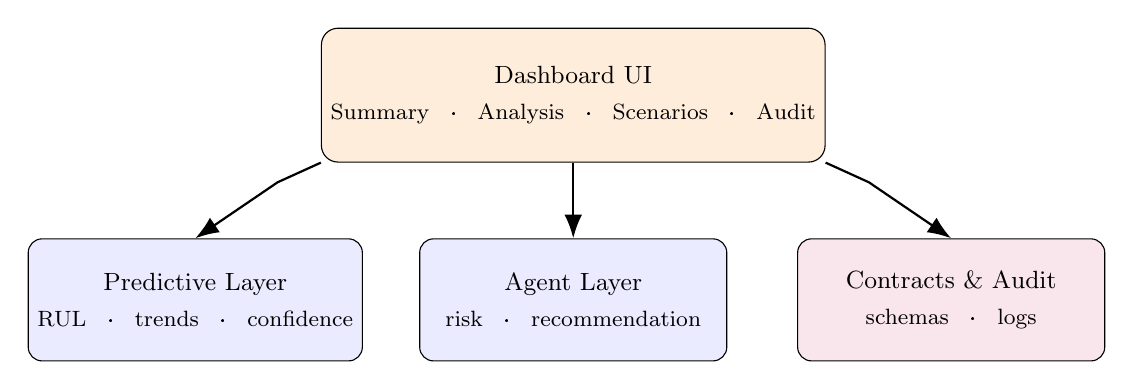
\begin{tikzpicture}[
  font=\small,
  >=Latex,
  main/.style={
    draw,
    rounded corners=6pt,
    minimum width=5.8cm,
    minimum height=1.7cm,
    align=center,
    fill=orange!14
  },
  layer/.style={
    draw,
    rounded corners=5pt,
    minimum width=3.9cm,
    minimum height=1.55cm,
    align=center,
    fill=blue!8
  },
  support/.style={
    draw,
    rounded corners=5pt,
    minimum width=3.9cm,
    minimum height=1.55cm,
    align=center,
    fill=purple!10
  },
  arrow/.style={
    -{Latex[length=3mm]},
    thick
  }
]

%---------------------------------
% Top node
%---------------------------------
\node[main] (dash) at (0,2.2)
{Dashboard UI\\[2pt]
{\footnotesize Summary \;\;·\;\; Analysis \;\;·\;\; Scenarios \;\;·\;\; Audit}};

%---------------------------------
% Bottom nodes
%---------------------------------
\node[layer]   (pred) at (-4.8,-0.4)
{Predictive Layer\\[2pt]
{\footnotesize RUL \;\;·\;\; trends \;\;·\;\; confidence}};

\node[layer]   (agent) at (0,-0.4)
{Agent Layer\\[2pt]
{\footnotesize risk \;\;·\;\; recommendation}};

\node[support] (audit) at (4.8,-0.4)
{Contracts \& Audit\\[2pt]
{\footnotesize schemas \;\;·\;\; logs}};

%---------------------------------
% Connections
%---------------------------------
\draw[arrow] (dash.south west) -- ++(-0.55,-0.25) -- (pred.north);
\draw[arrow] (dash.south) -- (agent.north);
\draw[arrow] (dash.south east) -- ++(0.55,-0.25) -- (audit.north);

\end{tikzpicture}

\caption{Simplified PHM architecture highlighting the dashboard as a multi-source consumer of predictive inference, agent-based decision logic, and audit infrastructure.}
\label{fig:architecture}
\end{figure}

\section{Experiments and Results}
\subsection{Global and per-dataset performance}
Table~\ref{tab:global_metrics} shows global metrics, while Table~\ref{tab:dataset_metrics} details subset behavior.

\begin{table}[H]
\centering
\caption{Global model metrics.}
\label{tab:global_metrics}
\begin{tabular}{lrrr}
\toprule
Model & RMSE & MAE & Rows \\
\midrule
GRU & 17.424 & 13.194 & 25,309 \\
RF & 18.313 & 13.256 & 32,267 \\
HGB & 18.433 & 13.329 & 32,267 \\
LSTM & 20.012 & 14.990 & 25,309 \\
\bottomrule
\end{tabular}
\end{table}

\begin{table}[H]
\centering
\caption{Per-dataset RMSE by model.}
\label{tab:dataset_metrics}
\begin{tabular}{lrrrr}
\toprule
Model & FD001 & FD002 & FD003 & FD004 \\
\midrule
GRU & 13.974 & 19.427 & 14.121 & 17.989 \\
RF & 18.686 & 19.600 & 16.978 & 17.512 \\
HGB & 18.680 & 19.763 & 17.065 & 17.654 \\
LSTM & 18.784 & 21.728 & 15.733 & 20.468 \\
\bottomrule
\end{tabular}
\end{table}

\begin{table}[H]
\centering
\caption{Latency and engineering trade-offs.}
\label{tab:latency}
\begin{tabular}{lrrr}
\toprule
Model & Samples & Total seconds & ms/sample \\
\midrule
HGB & 512 & 5.493 & 10.728 \\
RF & 512 & 0.161 & 0.313 \\
LSTM & 28,149 & 0.383 & 0.014 \\
GRU & 25,309 & 1.319 & 0.052 \\
\bottomrule
\end{tabular}
\end{table}

\subsection{Champion decision}
Although GRU obtains the best raw RMSE, the deployed champion remains RF due to stability and deterministic integration-readiness with an HGB fallback. This emphasizes application-level reliability over leaderboard-only optimization.

\subsection{Scenario and reliability evidence}
\begin{table}[H]
\centering
\caption{Scenario comparison example.}
\label{tab:scenario_example}
\begin{tabular}{lcc}
\toprule
Metric & Baseline & Scenario \\
\midrule
RUL prediction & 123.955 & 123.874 \\
Risk level & healthy & healthy \\
Risk score & 35 & 35 \\
Service status & ok & ok \\
\midrule
$\Delta$RUL & \multicolumn{2}{c}{-0.081} \\
$\Delta$Risk score & \multicolumn{2}{c}{0} \\
\bottomrule
\end{tabular}
\end{table}

\begin{table}[H]
\centering
\caption{Failure modes and handling.}
\label{tab:failure_modes}
\begin{tabularx}{\textwidth}{lX}
\toprule
Failure mode & Handling strategy \\
\midrule
Invalid request payload & Deterministic validation response with explicit error message \\
Predictive validation failure & Propagate \texttt{error\_validacion} service state \\
Champion unavailable & Use deterministic fallback model and state propagation \\
LLM key/provider failure & Continue with rules-only deterministic path \\
Unsafe scenario perturbation & Reject scenario with validation errors and safety notes \\
\bottomrule
\end{tabularx}
\end{table}

\begin{table}[H]
\centering
\caption{Contract and trace field mapping.}
\label{tab:contracts}
\begin{tabular}{lll}
\toprule
Dashboard tab & Field & Source layer \\
\midrule
Summary & \texttt{rul\_pred}, \texttt{risk\_level} & agent / predictive \\
Analysis & \texttt{risk\_score}, \texttt{confidence\_band}, \texttt{trace} & agent / predictive \\
Scenarios & \texttt{comparison}, \texttt{change\_summary} & agent scenario \\
Technical Audit & \texttt{audit\_record\_id}, \texttt{model\_version}, \texttt{service\_status} & agent / predictive \\
\bottomrule
\end{tabular}
\end{table}

\subsection{Dashboard evidence and visual results}
\begin{figure}[H]
\centering
\begin{subfigure}[b]{0.48\textwidth}
  \centering
  
\includegraphics[width=\textwidth]{dashboard_v1_3.png}
  \caption{Summary tab.}
\end{subfigure}
\hfill
\begin{subfigure}[b]{0.48\textwidth}
  \centering
  
\includegraphics[width=\textwidth]{dashboard_v1_5.png}
  \caption{Analysis tab.}
\end{subfigure}

\vspace{0.5em}
\begin{subfigure}[b]{0.48\textwidth}
  \centering
  
\includegraphics[width=\textwidth]{dashboard_v1_9.png}
  \caption{Scenarios tab.}
\end{subfigure}
\hfill
\begin{subfigure}[b]{0.48\textwidth}
  \centering
  
\includegraphics[width=\textwidth]{dashboard_v1_10.png}
  \caption{Technical Audit tab.}
\end{subfigure}
\caption{Dashboard evidence across operator and audit workflows.}
\label{fig:dashboard_suite}
\end{figure}

% \begin{figure}[H]
% \centering
% \begin{tikzpicture}
% \begin{axis}[
%     width=0.75\textwidth,
%     height=5cm,
%     ybar,
%     bar width=16pt,
%     ylabel={Cycles / score},
%     symbolic x coords={Baseline RUL,Scenario RUL,Delta RUL,Risk Score},
%     xtick=data,
%     x tick label style={rotate=20,anchor=east},
%     nodes near coords,
%     ymin=-1,
% ]
% \addplot coordinates {(Baseline RUL,123.955) (Scenario RUL,123.874) (Delta RUL,-0.081) (Risk Score,35)};
% \end{axis}
% \end{tikzpicture}
% \caption{Scenario comparison chart (F8) from deterministic baseline-vs-scenario outputs.}
% \label{fig:scenario_chart}
% \end{figure}

\begin{figure}[H]
\centering

\begin{subfigure}[t]{0.58\textwidth}
\centering
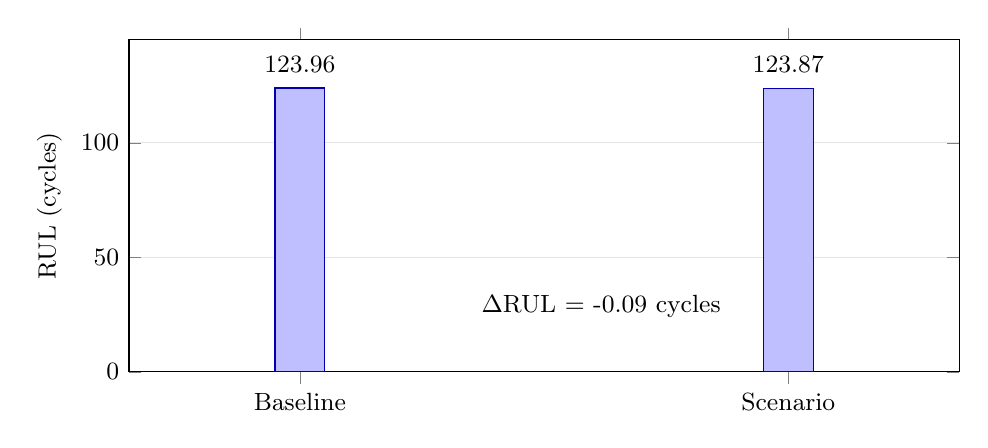
\begin{tikzpicture}
\begin{axis}[
    width=\textwidth,
    height=5.8cm,
    ybar,
    bar width=18pt,
    ymin=0,
    ymax=145,
    ylabel={RUL (cycles)},
    symbolic x coords={Baseline,Scenario},
    xtick=data,
    nodes near coords,
    every node near coord/.append style={
        font=\small,
        yshift=2pt
    },
    tick label style={font=\small},
    label style={font=\small},
    axis line style={black},
    enlarge x limits=0.35,
    grid=major,
    grid style={gray!20},
    ymajorgrids=true,
    xmajorgrids=false
]

\addplot[
    draw=blue!70!black,
    fill=blue!25
] coordinates {
    (Baseline,123.96)
    (Scenario,123.87)
};

\node[
    anchor=north east,
    font=\small,
    align=right,
    fill=white,
    fill opacity=0.9,
    text opacity=1,
    rounded corners=2pt,
    inner sep=2pt
] at (rel axis cs:0.72,0.25) {$\Delta$RUL = -0.09 cycles};

\end{axis}
\end{tikzpicture}
\caption{Baseline-versus-scenario RUL comparison.}
\label{fig:rul_compare}
\end{subfigure}
\hfill
\begin{subfigure}[t]{0.36\textwidth}
\centering
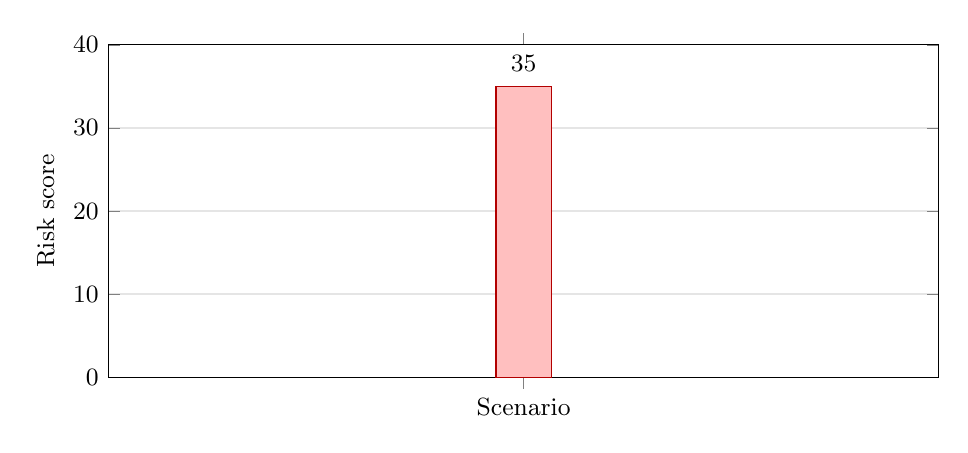
\begin{tikzpicture}
\begin{axis}[
    width=\textwidth,
    height=5.8cm,
    ybar,
    bar width=20pt,
    ymin=0,
    ymax=40,
    ylabel={Risk score},
    symbolic x coords={Scenario},
    xtick=data,
    nodes near coords,
    every node near coord/.append style={
        font=\small,
        yshift=2pt
    },
    tick label style={font=\small},
    label style={font=\small},
    axis line style={black},
    enlarge x limits=0.6,
    grid=major,
    grid style={gray!20},
    ymajorgrids=true,
    xmajorgrids=false
]

\addplot[
    draw=red!70!black,
    fill=red!25
] coordinates {
    (Scenario,35)
};

\end{axis}
\end{tikzpicture}
\caption{Scenario risk score.}
\label{fig:risk_score}
\end{subfigure}

\caption{Scenario comparison split into physical prediction and decision-oriented risk: (a) baseline and scenario RUL estimates with the associated $\Delta$RUL, and (b) the scenario risk score.}
\label{fig:scenario_chart}
\end{figure}

\begin{figure}[H]
\centering
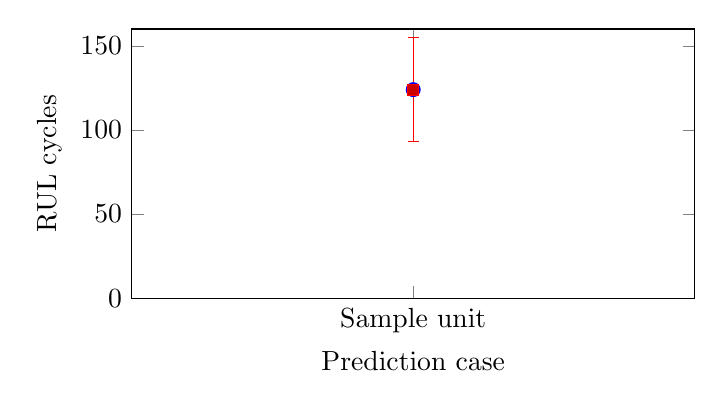
\begin{tikzpicture}
\begin{axis}[
    width=0.72\textwidth,
    height=5cm,
    xlabel={Prediction case},
    ylabel={RUL cycles},
    xtick={1},
    xticklabels={Sample unit},
    ymin=0,
    ymax=160
]
\addplot+[only marks, mark=*, mark size=2.5pt] coordinates {(1,123.955)};
\addplot+[error bars/.cd, y dir=both, y explicit] coordinates {(1,123.955) +- (0,31.0)};
\end{axis}
\end{tikzpicture}
\caption{RUL interval illustration using calibrated confidence-band policy around a point prediction.}
\label{fig:interval_plot}
\end{figure}

\section{Discussion}
The key engineering lesson is that the best benchmark model is not always the best deployed model. In this system, RF was selected over GRU to prioritize stable serving behavior, deterministic fallback, clear traceability, and low integration overhead. Scenario analysis further demonstrates that not all domain-meaningful perturbations produce large predictive effects if changes target excluded or locally insensitive features.

\section{Conclusion}
This work delivers a full PHM stack for C-MAPSS that integrates prediction, uncertainty, deterministic risk logic, scenario comparison, and auditability. Scientifically, it demonstrates calibrated RUL modeling with explicit champion-selection rationale. Engineering-wise, it demonstrates traceable end-to-end deployment with contract-driven boundaries and robust handling of degraded states.

\bibliographystyle{plain}
\bibliography{references}

\end{document}